% 原卷第11题正三棱锥；E,F 为 SC、AB 中点，底面后棱与 EF 用虚线。
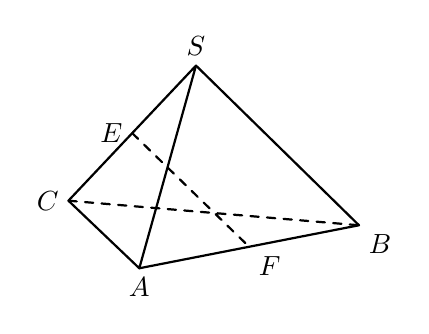
\begin{tikzpicture}[x=0.9cm,y=0.78cm,line cap=round,line join=round]
  \coordinate (S) at (0.8,3.3);
  \coordinate (A) at (0,0);
  \coordinate (B) at (3.1,0.7);
  \coordinate (C) at (-1.0,1.1);
  \coordinate (E) at (-0.1,2.2);
  \coordinate (F) at (1.55,0.35);
  \draw[thick] (S)--(A)--(C)--(S);
  \draw[thick] (S)--(B)--(A);
  \draw[thick,dashed] (C)--(B) (E)--(F);
  \node[above] at (S) {$S$};
  \node[below] at (A) {$A$};
  \node[below right] at (B) {$B$};
  \node[left] at (C) {$C$};
  \node[left] at (E) {$E$};
  \node[below right] at (F) {$F$};
\end{tikzpicture}
